\chapter{Introdução}

\section{Descrição do Problema e Estado da Arte}

Um grande desafio atual é promover a inclusão de pessoas com deficiências na sociedade, sejam elas quais forem. Tomando o caso dos deficientes visuais como foco, vários são os desafios enfrentados diariamente, desde a locomoção segura até o processo de aprendizado, ou mesmo o acesso à informação. Como uma forma de amenizar essas dificuldades, garantindo igualdade e promovendo a inclusão social e a cidadania daqueles que possuem alguma deficiência, o Congresso Nacional sancionou algumas leis nesse escopo.

Um exemplo é a Lei 13.146, sancionada em 2015, que instituiu o Estatuto da Pessoa com Deficiência. Em seu texto define acessibilidade em termos de possibilitar, dentre variados direitos, o acesso à informação e a garantia de autonomia para os deficientes. Além disso, trata também de tecnologia assistiva, que pode ser definida, resumidamente, como produtos, serviços ou estratégias que possibilitam ao deficiente a participação em determinada atividade, proporcionando-lhe independência, qualidade de vida e inclusão social \citeC{estatuto}.

Nessa perspectiva, \citeC{Bersch2013} também define tecnologia assistiva como o conjunto de recursos que amplia as habilidades daqueles que possuem alguma deficiência. Porém, \citeC{Bersch2013} vai além e assinala o que seria Tecnologia Assistiva em um contexto educacional ou informacional. Em um cenário no qual, antes, a participação ativa do estudante no processo de aprendizagem seria restrita ou praticamente inexistente, com a tecnologia assistiva a pessoa com deficiência poderia romper barreiras que limitam ou impedem o seu acesso à informação ou ao registro dela. Desta forma, favorecendo a participação e a autonomia do estudante em projetos, e por fim, provendo-lhe a manipulação dos objetos de estudo.

Ainda vale reforçar esse conceito, explicitando o ponto de vista sustentado por \citeC{Radabaugh1993} como segue na citação: ``Para as pessoas sem deficiência a tecnologia torna as coisas mais fáceis. Para as pessoas com deficiência, a tecnologia torna as coisas possíveis.''


No que tange à construção do conhecimento, segundo \citeC{Levy1993}, seu processo está fundamentado principalmente na oralidade e no desenvolvimento da linha de raciocínio durante a escrita do indivíduo. A elaboração do raciocínio, por sua vez, é composta e baseada nas informações acessadas e sentidas pelo sujeito em seu universo. No caso, portanto, do invidente, a informação e a conexão entre os diferentes conceitos aprendidos se dá de forma distinta dos videntes, uma vez que esse processo encontra-se sempre dependente da capacidade do indivíduo de construir significado por meio dos sentidos \citeC{Neto2006}. Sendo assim, é fácil concluir que são sujeitos que necessitam de uma abordagem cuidadosa quanto ao consumo de informação.

Um exemplo claro da necessidade de adequação de material para estudo dos deficientes visuais é o caso do campo de estudos denominado STEM, acrônimo em inglês para Ciências, Tecnologia, Engenharia e Matemática. Os problemas enfrentados são vários, começando com a dificuldade presente no próprio ambiente de estudo, já que, para que adaptações em infraestrutura sejam feitas, os gastos para a universidade seriam consideráveis. Consequentemente, esses ajustes necessários para o bom processo de aprendizagem dos deficientes visuais são constantemente negligenciados. Além disso, muitos professores e colegas não são familiarizados quanto ao proceder em relação aos estudantes invidentes. Porém, provavelmente o problema com maior impacto é a falta de material em si que seja acessível, contendo informações gráficas importantes e que muitas vezes são imprescindíveis ao ensino nessa área. Uma alternativa seria, por exemplo, utilizar técnicas multissensoriais para experimentos científicos, tecnologias com \textit{design} apropriado, como modelos 3D ao invés de figuras em livros, e também softwares que transformam imagens em conteúdo audível \citeC{Beck-Winchatz2008}.

Graças a alguns estudos e projetos que vem sendo desenvolvidos, percebe-se que os deficientes visuais totais ou parciais tem um grande proveito no processo de aprendizagem ao combinar recursos hápticos com instruções ou acompanhamento sonoro. No caso, por exemplo, do sistema apresentado por \citeC{Plimmer2008}, estudantes são ensinados a assinarem o próprio nome por meio de instruções de áudio que lhes são passadas, enquanto sentem por meio do tato a sua própria assinatura em alto relevo e em tempo real. Desta forma, conseguiu-se um resultado mais significativo do que apenas ensiná-los sem o auxílio combinatório desses dois recursos. Além desse trabalho, há também o ensino de desenho à deficientes visuais em cujo processo são empregadas diferentes sensações táteis, como a diferença de relevo e textura e também os sons. O autor destaca como esses e outros componentes sensoriais, como exemplo, a temperatura, afetam o deficiente visual, fazendo-o perceber, de maneira indireta, aspectos distintos em um ambiente \citeC{Ballestero-Alvarez2003}.

No entanto, é extremamente necessário que um fato fique claro, as imagens mentais que os invidentes constroem do mundo que os rodeia são semelhantes àquelas criadas pelo indivíduo comum, apesar de serem formadas de maneiras distintas \citeC{Soler1999}. Na ausência de um dos sentidos, a percepção do ambiente e dos objetos vem a partir dos demais sentidos. Por isso, para o deficiente visual, é essencial que eles estejam conectados durante o processo de aprendizagem, de forma que possa-se extrair mais informações visuais sobre o objeto de estudo por meio da multissensorialidade \citeC{Ballestero-Alvarez2003}.

Sendo assim, é de suma importância que, para o estudo de determinado objeto, a adaptação da informação visual seja feita de acordo com o sentido mais apropriado para cada caso. Esse conceito é muito bem exemplificado por \citeC{Ballestero-Alvarez2003}, quando fala sobre a torre Eiffel sendo apresentada a estudantes invidentes em ambientes de estudo. Nesse caso, a opção mais interessante seria além de disponibilizar-lhes uma maquete, a abordagem mais óbvia, descrever-lhes também a estrutura da torre e seus detalhes, para que assim a experiência de aprendizado seja mais completa, harmonizando os sentidos, a fim de proporciona-lhes uma melhor imagem mental.

Outro ponto que suporta essa argumentação é que, em muitos casos, a imagem mental formada por videntes não é composta somente por aspectos visuais, mas envolve também outros sentidos de forma simultânea. Logo, a construção do conhecimento de algum objeto para os deficientes visuais, apesar de poder ser em um ritmo distinto do que o é para os videntes, não é, de forma alguma, incompleta ou inferior, sendo ainda mais desenvolvida quando possuem adaptações adequadas para cada caso \citeC{Ballestero-Alvarez2003}.

Portanto, é fácil perceber a importância de plataformas, produtos, serviços ou metodologias que se adequem à realidade do deficiente visual e proporcionem o envolvimento com áreas do conhecimento antes inexploradas por eles, ou então que os capacitem a exercer funções ou realizar tarefas que antes eram impossíveis. Atualmente, ainda que de forma limitada, há esforço por parte de alguns para que a realidade de exclusão de deficientes seja mudada e que a inclusão se torne cada vez mais presente na vida deles.

Nesse sentido, podem-se ressaltar alguns trabalhos em desenvolvimento ou já desenvolvidos com esse propósito de acessibilidade. No Museu de Arte da Universidade Federal do Paraná (MusA), foi realizada uma exposição voltada para o público deficiente visual com a transposição de imagens em peças táteis, utilizando materiais para realçar linhas de contorno. Nesse projeto foram desenvolvidos materiais, em braille e ampliados, de apoio didático sobre as obras de arte e sobre o museu, além de uma sessão de treinamento para os deficientes visuais anterior à sua visita, de forma a melhor ambientá-los e possibilitar a formação de uma imagem mental prévia, potencializando assim a experiência durante a exposição \citeC{Fernanda2007}.

Uma plataforma que se destaca bastante é o \textit{DOSVOX}, desenvolvido pela Universidade Federal do Rio de Janeiro \citeC{Borges1998}. O \textit{DOSVOX} consiste em um sistema operacional que possibilita ao deficiente visual o uso do computador para realização de variadas tarefas. Esse sistema se tornou uma ferramenta muito importante para a inclusão dos invidentes, utilizada em todo o Brasil, destacando-se por ser uma ferramenta gratuita. O \textit{DOSVOX} inclui alguns jogos didáticos, a tradução do Braille para a escrita romana e vice-versa, a leitura de textos por meio de síntese de voz, a composição e a impressão de partituras e entre outras funcionalidades \citeC{Amorim2009}.

Outras tecnologias assistivas que se destacam são o \textit{Jaws} e o \textit{Virtual Vision}, sendo ambos são softwares leitores de tela para uso em computador \citeC{Jaws2016} \citeC{VV2016}. Nesse mesmo escopo existe o software \textit{OpenBook} que escaneia documentos impressos, digitaliza-os e os lê e dá instruções em áudio para o deficiente visual o operar \citeC{OpenBook2016}. Também foi desenvolvido um dispositivo chamado Linha Braille ou \textit{Display} Braille que, quando conectado ao computador, exibe dinamicamente a informação da tela em braille e que possui também botões adicionais para controle dos softwares leitores de tela, unindo a informação sonora à leitura tátil \citeC{Linha2008}. Outra ferramenta bastante interessante é o \textit{TactileView for Tactile Graphics}, que consiste em um software para impressão de figuras e gráficos com pontos em alto relevo \citeC{Tactile2016} \citeC{Amorim2009}.

Porém, apesar de toda essa variade de ferramentas desenvolvidas até hoje, pouco material foi disponibilizado acerca do ensino da tipografia para deficientes visuais. O trabalho que talvez se aproxime mais dessa proposta é o sistema de \citeC{Plimmer2008}, que tem como objetivo ensinar de maneira mais eficaz os deficientes visuais a escrita à mão, começando com a assinatura de seu próprio nome. No entanto, seu foco é apenas nos caracteres, na escrita em si, e não na tipografia envolvida.

Um outro exemplo que envolve essa área, é o projeto de tipografia ajustável. O sistema possibilita aos deficientes visuais com baixa visão customizar parâmetros da fonte utilizada no documento para melhorar sua legibilidade, de acordo com a necessidade de cada indivíduo \citeC{Arditi2004}. Entretanto, a tipografia é envolvida nesse caso como uma ferramenta para possibilitar a leitura e não como objeto de estudo. Apesar de o software possibilitar a percepção da diferença causada pela variação dos parâmetros do tipo, o contato com os conceitos da tipografia é nada mais do que empírico e pragmático nesse caso.

A tipografia, assim como a caligrafia e a escrita, serve para comunicação, podendo ser direta ou indireta. Assim como em várias formas de arte, a tipografia tem seu papel principal na comunicação indireta, comunicando por meio de formas e criando uma linguagem visual. Ao associar o significado das palavras à essa linguagem, a interpretação é gerada. Se o deficiente visual é privado dessa informação transmitida por meio da linguagem visual criada pela tipografia, ele é também privado de parte da mensagem transmitida, caracterizando uma comunicação que não é bem sucedida em seu todo \citeC{Velasco2015}.

Sensações também são geradas por meio da tipografia. Nesse caso, apesar de o fim principal ser sempre a comunicação, a questão visual e estética pode ser mais importante do que o conteúdo das palavras em si, aproximando-se ainda mais do campo das artes no sentido de forma de comunicação. Dessa maneira, o deficiente visual é ainda mais prejudicado quando privado dos detalhes da área, já que grande parte da mensagem não se encontra no sentido das palavras ali escritas. Por gerar sensações distintas, uma das aplicações mais importantes da tipografia é diferenciar estilos, produtos e marcas. Nesse sentido, o deficiente visual também é bastante prejudicado quando não tem contato com todo esse universo de logotipos, marcas, filmes, bandas, entre outros campos no quais é aplicada a tipografia e nos quais os videntes estão imersos \citeC{Velasco2015}.

Além disso, a tipografia também tem relevância no campo histórico, no qual influencia e pelo qual é influenciada. Um exemplo para clarear esse conceito é o evento da invenção da imprensa. Antes de sua criação, a comunicação e o acesso à informação eram bastante exclusivistas pois, apenas poucas pessoas sabiam escrever e tinham acesso a esse tipo de material como, por exemplo, os monges. Porém, com o advento da imprensa e, consequentemente, da tipografia, houve um crescimento exponencial da comunicação e da distribuição do conhecimento por meio da escrita, inclusive a Reforma Protestante aconteceu em grande parte baseada nesse advento \citeC{Costa2008}. Por esse aspecto, a tipografia foi essencial para a disseminação do conhecimento. Em outra perspectiva, ela também foi influenciada, já que, naquela época, os tipos eram todos físicos e as características daquela tipografia eram moldadas pelo material que era utilizado para sua produção. Ela sofre influências até hoje, como qualquer área do conhecimento, mas principalmente no campo artístico, no qual as suas características mais acentudas são moldadas por uma filosofia da sociedade da época \citeC{Kane2012} \citeC{Rodrigues2012}.



\section{Proposta de Projeto}

Tendo esses pontos em vista, propõe-se um sistema para ensino de tipografia para deficientes visuais. Abre-se, então, a oportunidade de um novo tipo de leitura. Um novo horizonte de conhecimento e interação dos invidentes com os caracteres romanos, usados em mais de um terço do mundo \citeC{World2015}. \citeC{Neto2006} faz um trabalho voltado para responder a questão sobre qual é a influência que o uso das tecnologias assistivas de informação e comunicação tem sobre a experiência do deficiente visual com a escrita e com a leitura por meio do braille. No entanto, a proposta aqui apresentada estende esse objetivo, desejando conectar o deficiente visual a um conceito mais robusto e completo. Pretende-se inseri-lo em um contexto que diz respeito não somente aos caracteres utilizados pela língua nativa do país onde vive, ou seja, do universo que o envolve, mas também criar nele um senso do que é a anatomia de cada letra, diferenciando os caracteres em si e também os diferentes tipos, aproximando-o da experiência que um vidente tem ao ler qualquer mídia, uma vez que em todas elas está empregada a tipografia.

Os deficientes visuais se encontravam em um "gueto cultural" antes do desenvolvimento de ferramentas como o \textit{DOSVOX} que possibilitassem a tradução dos textos escritos em braille para os caracteres romanos. Suas produções ficavam restritas já que raros videntes sabem ler ou escrever em braille, e o acesso à informação também ficava comprometido \citeC{Borges1998}. Nesse sentido, o projeto aqui proposto contribui também para a extinção de um "gueto cultural", entretanto fazendo um processo distinto, que é a aproximação dos deficientes visuais à escrita latina.

Além disso, o sistema possui não só um caráter de aproximação do invidente com a escrita e com os diversos estilos tipográficos, proporciona-lhe também a opção de se aprofundar em termos de estudo, se assim desejar, da tipografia com seus conceitos, aplicações e contextos históricos. Sendo assim, esse projeto caracteriza-se como um material inédito, no sentido de ser uma tecnologia assistiva que proporciona ao invidente o contato com uma informação antes restrita a ele, possibilitando o aprendizado de um ramo antes inexplorado por deficientes visuais e entregando-lhe em mãos um arsenal de novas informações, apesar de inicialmente ainda ser uma tecnologia com opções limitadas.


Além do mais, como o envolvimento dos deficientes visuais com o mundo digital da informática está crescendo, segundo \citeC{Neto2006}, há necessidade de cursos formativos para que o invidente saiba se enteirar melhor de todas as suas possibilidades de leitura e escrita com o apoio das tecnologias assistivas desse naipe. Sendo assim, o maior contato com a tipografia é um fator presente nesse complexo informativo e que deve ser ensinado ao deficiente visual, tendo em vista que esse é um campo intrínseco em mídias digitais textuais e, para os invidentes, por não ser-lhes dado acesso ao ensino da tipografia, ainda é uma área de desconhecimento e dúvidas.

A proposta para esse projeto foi idealizada primeiramente pela estudante de \textit{Design} Luciana Cruz, da Universidade de Brasília  na disciplina de Projeto de Produto 2, na qual foi orientada a propor e desenvolver um produto que viabilizasse acessibilidade a qualquer pessoa com deficiência. A proposta realizada ao final da disciplina foi um sistema para ensino de tipografia a deficientes visuais, que consiste em placas tridimensionais de MDF com as letras de 250 pontos inseridas em alto relevo, que podem ser vistas na Figura \ref{fig:dt}. Esse sistema provê ao deficiente visual a identificação minuciosa das características anatômicas e estilísticas de variados tipos, contando com o alfabeto completo para cada tipografia e também com um sistema pedagógico para que os deficientes visuais possam compreender as nuances e sutilezas da variedade de fontes tipográficas da escrita latina, entendendo seus significados formais e históricos \citeC{Cruz2016}.

%\begin{figure}[h]
%\caption{Desenho Técnico da Placa "A" Helvetica}

%\label{figura:dt}
%\end{figure}

\begin{figure}[H]
  \centering
  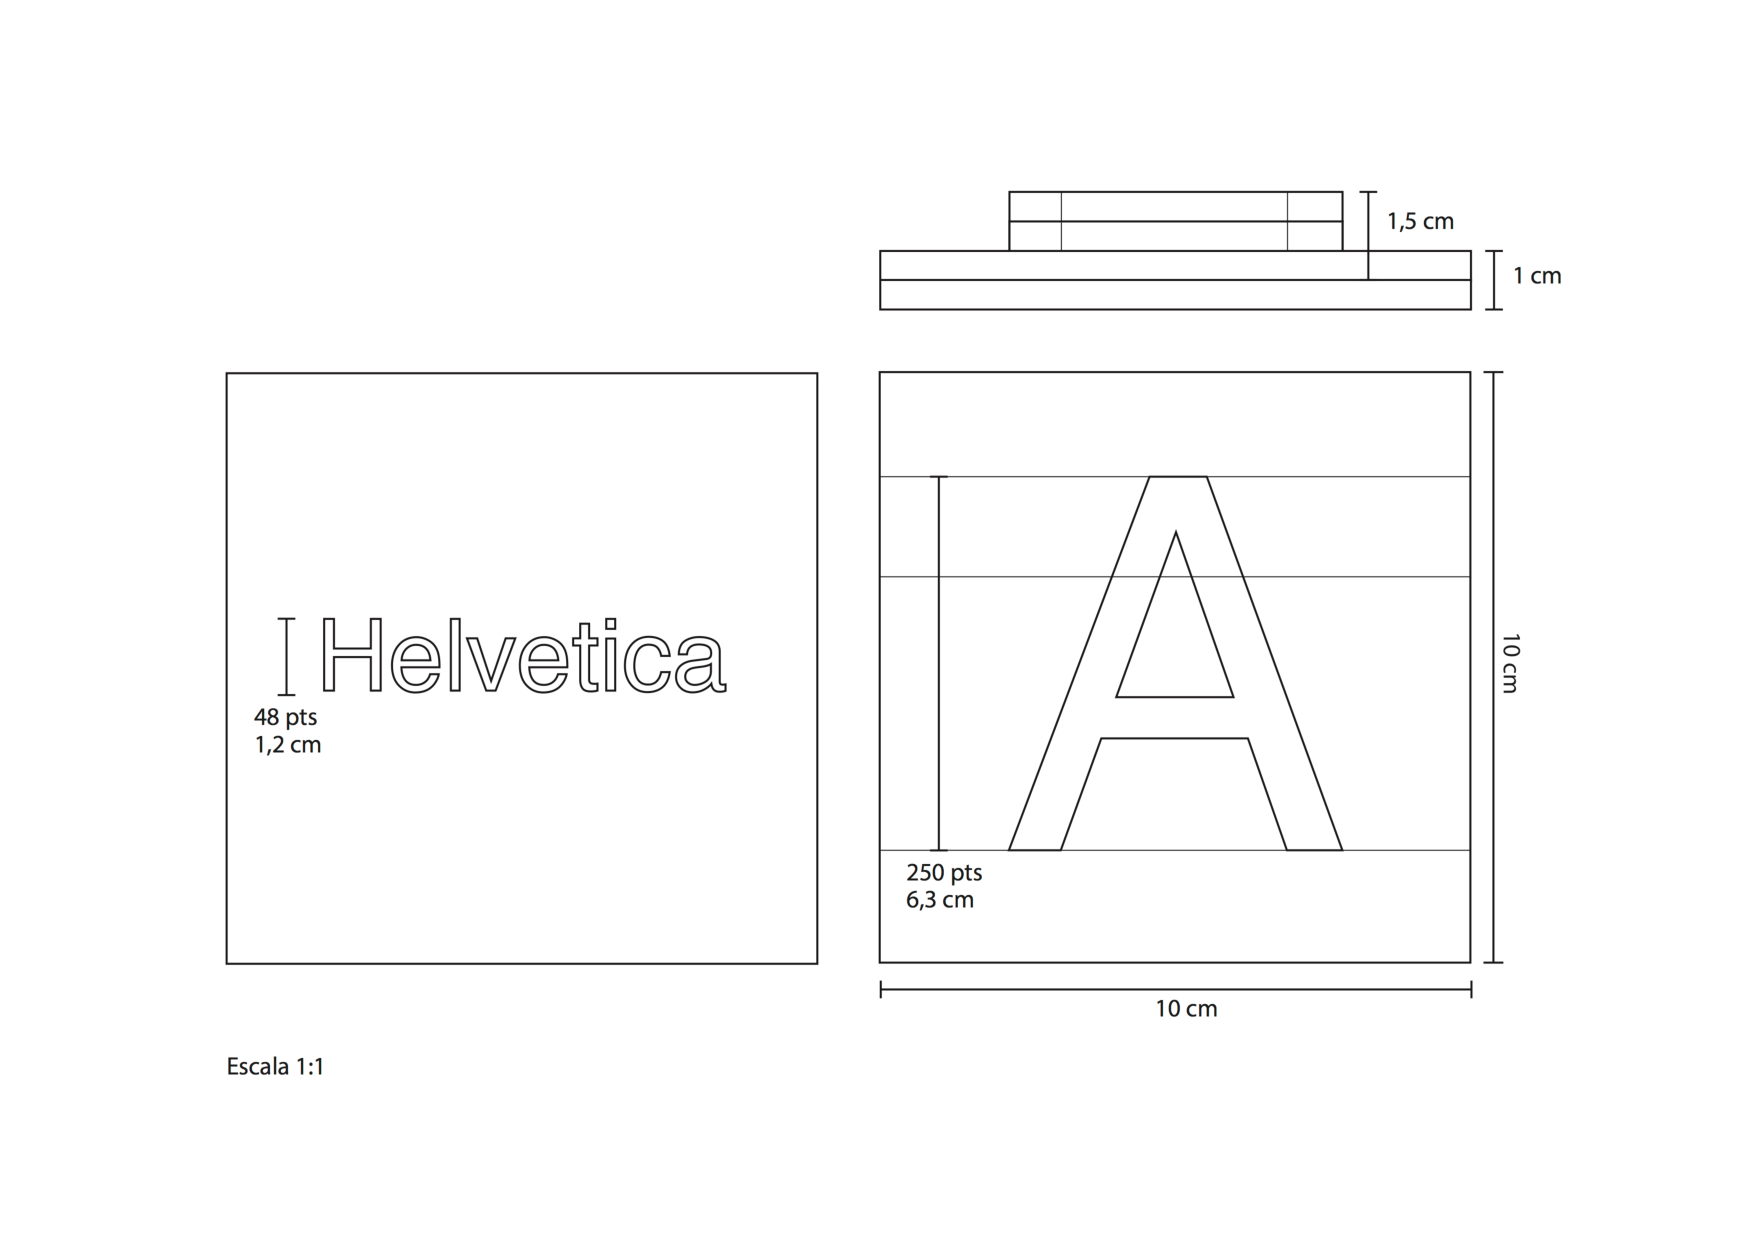
\includegraphics[width=0.7\linewidth]{figuras/DT-press-start.pdf}
  \caption{Desenho Técnico da Placa "A" Helvetica - \textbf{Fonte:} \citeC{Cruz2016}}
  \label{fig:dt}
\end{figure}

De modo a tornar o sistema ainda mais completo, com o intuito de proporcionar ao deficiente a autonomia ao estudar, como prevê o conceito da tecnologia assistiva, propôs-se a implementação de um sistema para reconhecimento de padrões nos tipos e para a classificação automática de qual tipografia o deficiente visual está manuseando, além de qual caractere. Por meio então da síntese de voz, serão providas ao usuário informações detalhadas sobre a teoria envolvida naquela tipografia, desde os conceitos básicos de anatomia até suas aplicações, especificações estilísticas e contexto histórico, compondo assim a ação pedagógica. Vale ressaltar que a implementação desse sistema garante o estudo por meio da multissensorialidade, que é uma técnica de maior eficácia no aprendizado dos deficientes visuais, como já discutido.

O fundamento do reconhecimento de padrões é o descobrimento de regularidades em dados por meio do uso de algoritmos computacionais e, então, a classificação desses dados em categorias. Logo, essa técnica provê o resultado necessário para tal aplicação. O reconhecimento de padrões em dados é uma técnica vital para a ciência desde muito tempo atrás. Um exemplo, é o progresso da física quântica no século XX, que se desenvolveu baseando-se, em grande parte, na descoberta de padrões no espectro atômico \citeC{Bishop2006}.

Para o reconhecimento de padrões, serão empregadas técnicas de Aprendizado de Máquina (\textit{Machine Learning}). Geralmente essa é a melhor abordagem para se tratar problemas de reconhecimento de padrões, apesar de também haver a possibilidade de serem aplicadas outras técnicas como as heurísticas, porém apresentam resultados insatisfatórios. O funcionamento desse sistema se dá, primeiramente, com a composição de um grande conjunto de dados que forma o conjunto de treinamento (\textit{training set}). Esses dados serão referências nas quais o computador irá se basear para regular os parâmetros do modelo adaptativo que será usado posteriormente para classificação do que se deseja reconhecer, no caso, os tipos \citeC{Bishop2006}.


Nesse caso, as categorias dos dados já são previamente conhecidas e rotuladas, sendo elas o nome de cada tipografia. Portanto, trata-se de uma situação na qual o processo de aprendizado de máquina é denominado um problema de conhecimento controlado (\textit{supervised learning}), sendo assim essa abordagem não é a mais complicada no cenário de reconhecimento de padrões. Então, após a execução do algoritmo de aprendizado de máquina, o resultado retornado é uma função que recebe como entrada um dado, nesse caso, a imagem de um tipo, e gera um vetor-alvo, que representa a categoria daquele dado. A forma dessa função é construída durante a sessão de treinamento ou de aprendizagem do algoritmo, baseada no banco de dados que forma o conjunto de treinamento \citeC{Bishop2006}.

Posterior à essa fase, o algoritmo já consegue identificar a categoria de um conjunto de novas imagem de entrada, denominado conjunto de teste. Porém, em muitas aplicações, mesmo após todo esse processo, devido à grande variação dos dados de entrada, o algoritmo consegue compreender apenas uma pequena porção de todo o conjunto que deseja-se classificar. Sendo assim, uma prática comum é passar os dados por um método de pré-processamento, de forma a aumentar a uniformização entre as imagens de entrada. Um exemplo do processo adotado em um algoritmo de reconhecimento óptico de caracteres (OCR, \textit{Optical Character Recognition}, em inglês) é mostrado na Figura \ref{fig:etapas}, que é uma abordagem comum para a resolução desse tipo de problema, sendo um caso semelhante ao aqui proposto \citeC{Bishop2006} \citeC{Miranda2013}.
%%%%

\begin{figure}[H]
  \centering
  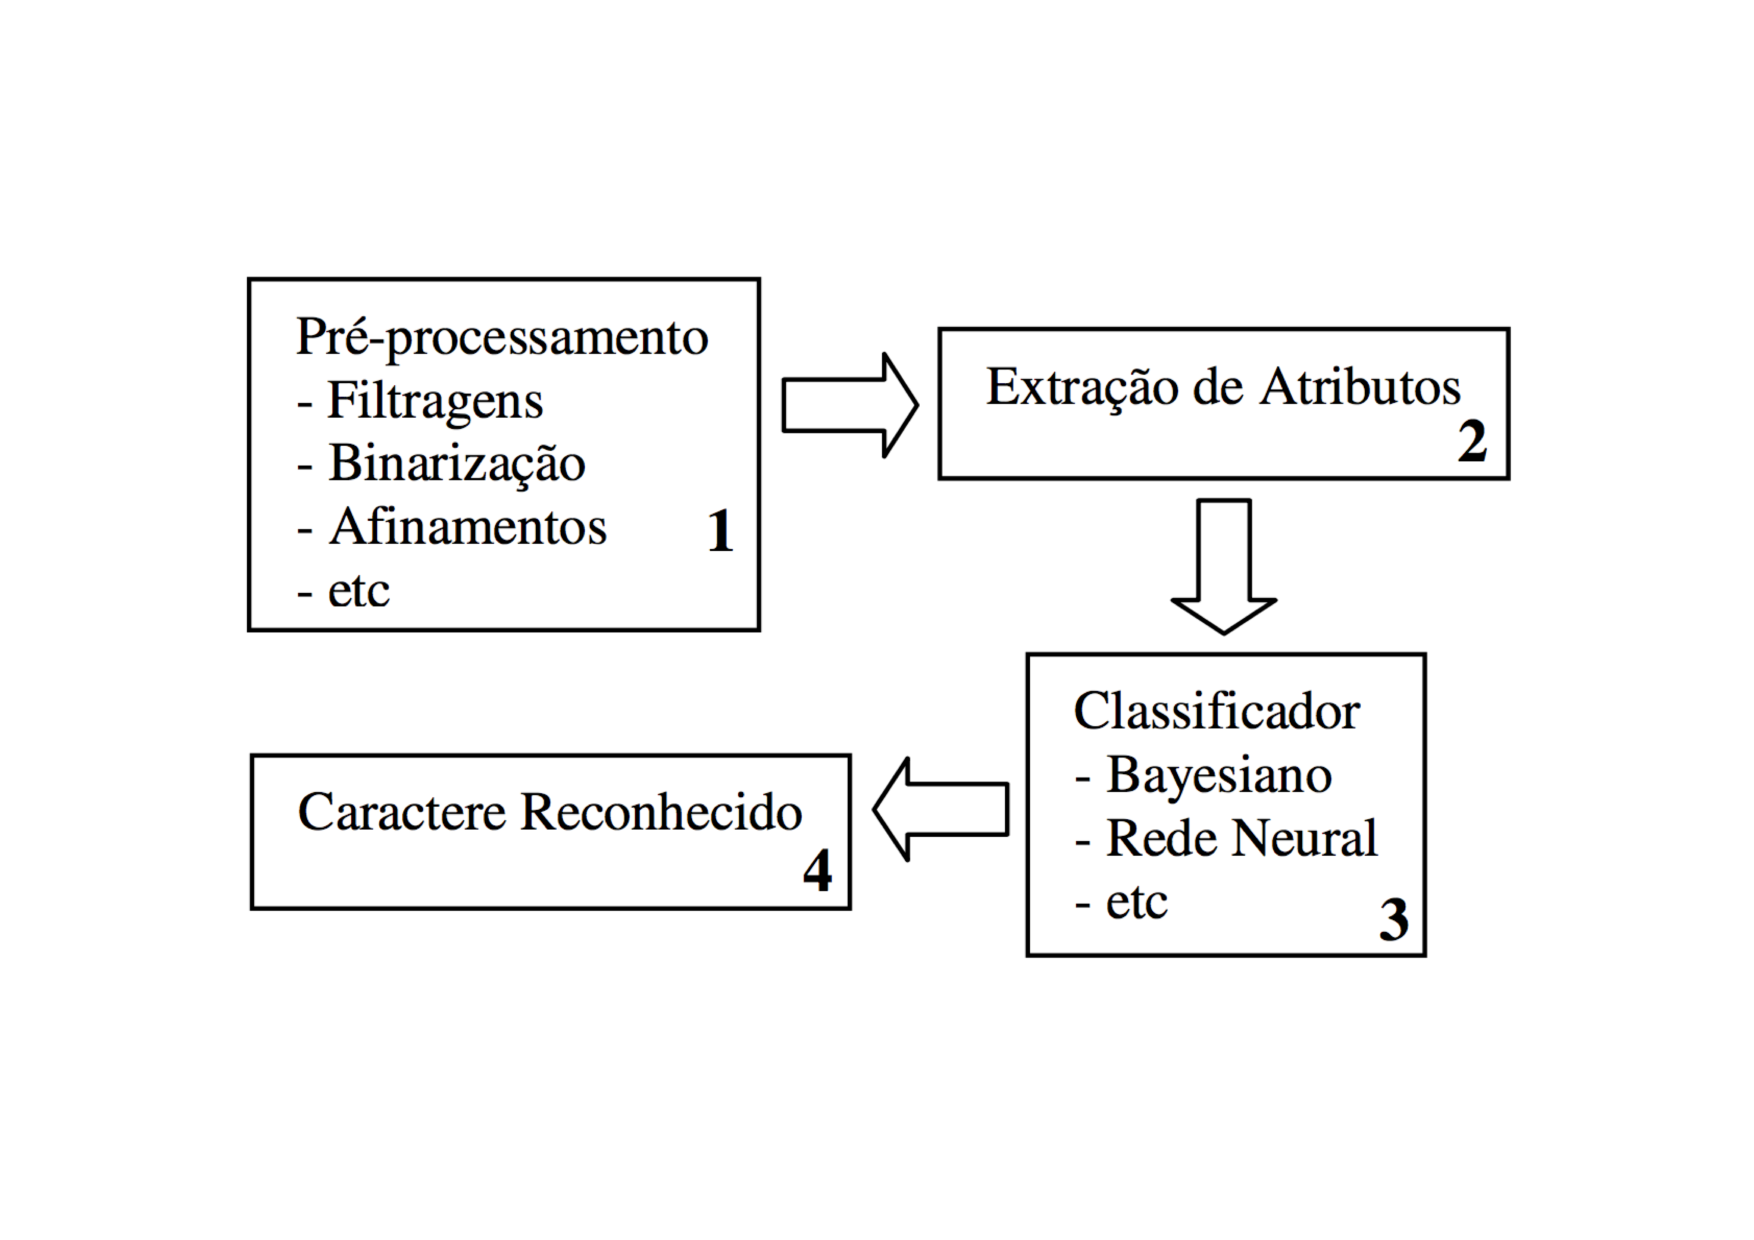
\includegraphics[width=0.7\linewidth]{figuras/etapaProcessamento.pdf}
  \caption{Etapas do Processo de Reconhecimento de Caracteres - \textbf{Fonte:} \citeC{miranda2013handwritten}}
  \label{fig:etapas}
\end{figure}

Vários dos softwares de tecnologia assitiva utilizam OCR em sua composição para leitura de tela ou de arquivos, como o \textit{OpenBook}, o \textit{Jaws} e o \textit{Virtual Vision} \citeC{OpenBook2016} \citeC{Jaws2016} \citeC{VV2016}. No sistema de auxílio ao ensino da escrita à mão para deficientes visuais, \citeC{Plimmer2008} também utiliza OCR e uma abordagem semelhante à de \citeC{Miranda2013}. Desta forma, percebe-se que esse campo de reconhecimento de caracteres vem favorecendo bastante o desenvolvimento de várias tecnologias e, em especial, as assistivas e também será utilizado para o reconhecimento de qual caractere o deficiente visual está utilizando durante a interação com os tipos táteis do sistema.

Apesar de o reconhecimento de padrões ter raízes históricas na ciência, a sua abordagem a partir do aprendizado de máquina encontra-se em um momento ímpar de crescimento. Graças ao veloz crescimento e popularização dos dispositivos com câmera, como smartphones e tablets, e também da internet e redes sociais, o volume de imagens e vídeos compartilhados na rede é imenso. Além disso, a capacidade de processamento dos computadores também apresenta um crescimento acelerado. Dessa forma, o aprendizado de máquina enfrenta um ótimo momento  para seu desenvolvimento, já que está acessível um grande banco de dados de imagens para compor o conjunto de treinamento e, além disso, as requisições de hardware para o processamento também \citeC{Feris2016}. Sendo assim, várias são as aplicações nessa área, desde utilidades no campo das ciências sociais até o campo da criminalistica \citeC{Grimmer2015} \citeC{li2015clothing}. Para o reconhecimento de padrões na Visão Comuputacional, o aprendizado de máquina é muito importante, sendo aplicado em várias situações como, por exemplo, localização de prédios, reconhecimento facial e edição inteligente de fotos \citeC{szeliski2010computer}.

Porém, o reconhecimento de tipos (OFR, \textit{Optical Font Recognition}, em inglês) continua um campo não amplamente explorado pela comunidade de pesquisadores \citeC{Zramdini1995}. Geralmente, quando o problema é atacado, utiliza-se o reconhecimento de tipos apenas para alguma forma de melhoria no processo de reconhecimento de caracteres quando se trata de um documento com variadas tipografias ou para uma possível classificação de documentos que diferenciados de acordo com a tipografia ali empregada, mas não como foco em si \citeC{Shi1997} \citeC{Manna1999}. Outra situação na qual aplica-se o reconhecimento de fontes é com o intuito de possibilitar o reconhecimento de caracteres não-latinos, como chineses, arábicos ou farsi \citeC{Yang2006} \citeC{Slimane2013} \citeC{Zahedi2011}.

No entanto, nesse contexto, o trabalho de \citeC{Zramdini1995} se destaca por desenvolver um sistema que considera todas as variedades anatômicas e intrafamiliares das fontes e por também propor uma combinação entre o reconhecimento de fontes e de caracteres, o que faz parte do objetivo do sistema final proposto para o projeto. Na Figura \ref{fig:OFRareas} pode-se ver a combinação de todas as áreas necessárias para o reconhecimento de fontes, essa abordagem apresentada por \citeC{Zramdini1995} será de grande valia nesse projeto.

\begin{figure}[H]
  \centering
  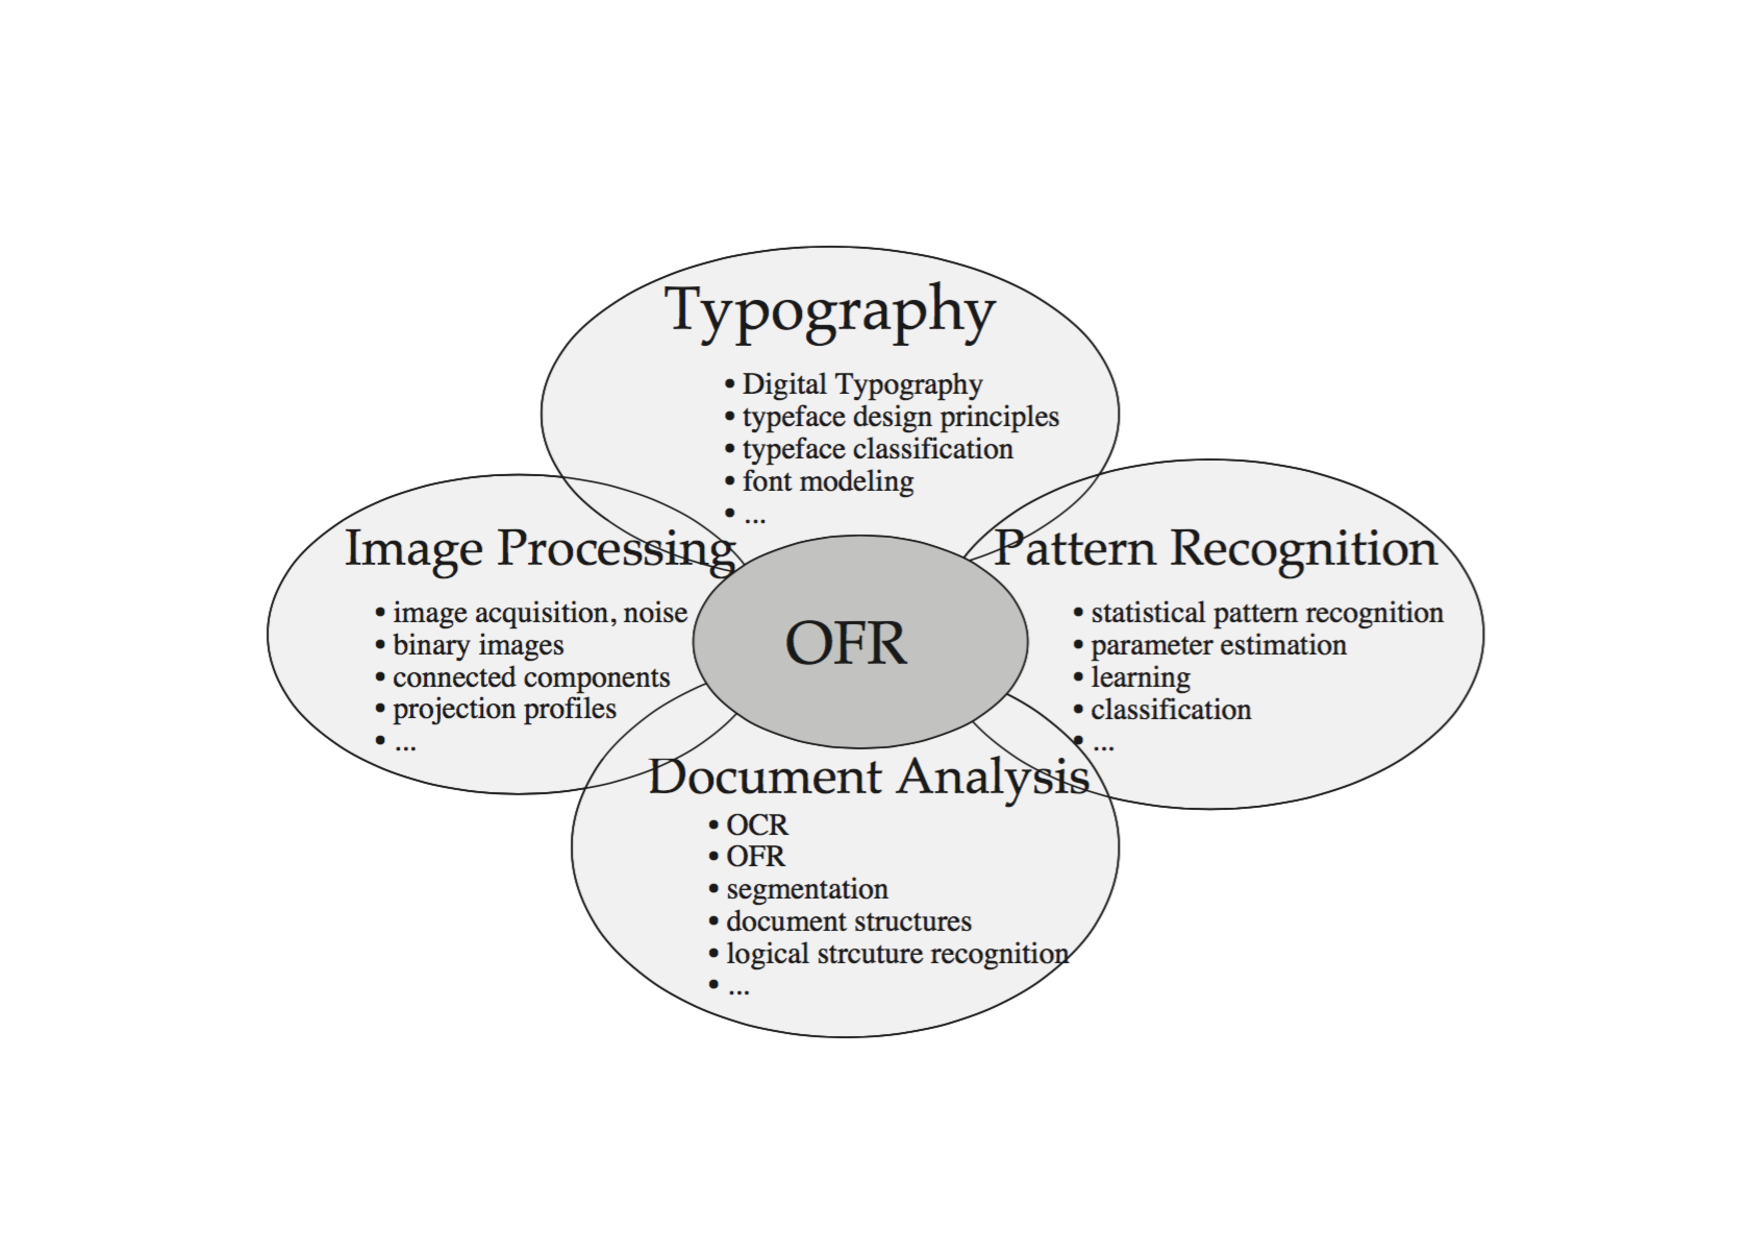
\includegraphics[width=0.8\linewidth]{figuras/OFRareas.pdf}
  \caption{Áreas Necessárias para Reconhecimento de Fontes - \textbf{Fonte:} \citeC{Zramdini1995}}
  \label{fig:OFRareas}
\end{figure}



%for the recognition of characters, but the rec- ognitionofthetypeoffontsisdisregarded \citeC{aviles2005}
%The methodology applied in our processing im- age algorithm was based on to estimate features not over full image, instead of this, feature estima- tionwasdoneoverregionsofimagescalled‘‘sub- image’’.Theestimatedattributearraysofeach sub-image were the reference database to recognize thetypeofeachfont(100windowsaretakenran- domlyovereachfulltext) \citeC{aviles2005}



%Uma citação~\cite{artigo:2015}.

%As citações são feitas usando o comando~\texttt{\textbackslash cite}. Para usar colchetes nas citações, use o comando~\texttt{\textbackslash citeC}. Exemplo \citeC{artigo:2015}.


%blá blá, blá \cite{artigo:2015}
